%%%%%%%%%%%%%%%%%%%%%%%%%%%%%%%%%%%%%%%%%
%
% N-CUBES
%
%%%%%%%%%%%%%%%%%%%%%%%%%%%%%%%%%%%%%%%%%

\section{Higher dimension intervals}

For now, we will concern ourselves only with oriented, $n$-dimensional, axis-aligned rectangles in $\mathbb{R}^n$.
In one dimension, the previously discussed oriented intervals cover most of the ``obvious shapes'' one would be interested in.
Moving to two dimensions, there are many more ``obvious shapes'' to consider but we will temporarily ignore triangles, circles and even rectangles that are tilted.
We could also use triangles instead of rectangles as our primitive of choice. 
This would generalize to $n$-simplexes in higher dimensions.
Since $n$-simplexes and $n$-cubes end up b\cite{choquetanalysis}
But, first we must introduce some notation to describe these and higher dimension rectangles. 

At the moment the only rectangles we have defined are the one-dimensional ``oriented interval''.
Hence we will also refer to this as a 1-cube.
We construct higher dimensional $n$ rectangles using the Cartesian product.
\begin{definition}
	Let $X = \hset{ x_1^{m_1}, ... , x_k^{m_k} }$ and $Y= \hset{ y_1^{n_1}, ... , y_\ell^{n_\ell} }$ be hybrid sets.
	We define the \textbf{Cartesian product of hybrid sets $\boldsymbol{X}$ and $\boldsymbol{Y}$}, denoted with $\times$ operator as:
	\begin{equation}
		X \times Y = \hset{ (x, y)^{m \cdot n} \; : \; x \in^m X, y \in^n Y }
	 \end{equation}
\end{definition}

If $[\![a,b]\!]$ and $[\![c,d]\!]$ are both positively oriented 1-rectangles then their Cartesian product is shown in Figure 4.1 is clearly a two dimensional rectangle or \emph{2-rectangle}. 
Taking the Cartesian product of a 2-rectangle and 1-rectangle gives a 3-rectangle in $\mathbb{R}^3$. 
We should note here that we do not distinguish between $((x,y),z)$ and $(x,(y,z))$ but rather we treat both as different names for the ordered triple $(x,y,z)$.
We similarly associate parentheses in higher dimensions as well.

\begin{figure}[ht]
\caption[Cartesian product of two 1-rectangles]{The Cartesian product of two positively oriented 1-rectangles $[\![a,b]\!]$ and $[\![c,d]\!]$ is a positively oriented 2-rectangle.}
\centering
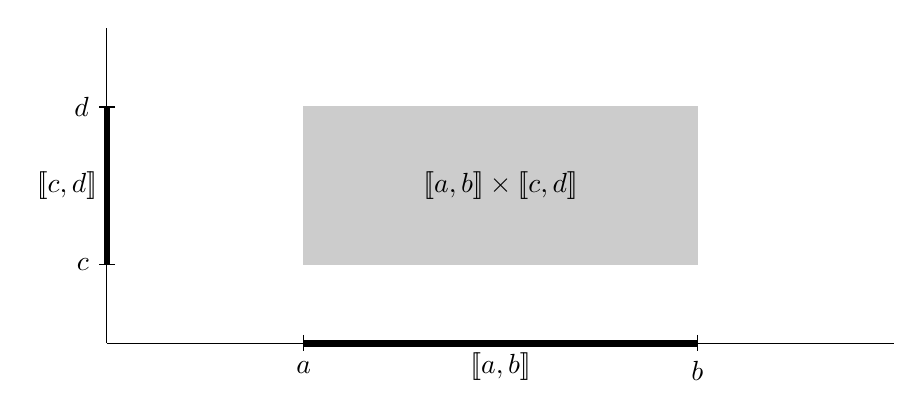
\begin{tikzpicture}[y=1cm, x=2.5cm]	
 	%axis
	\draw(0,0) -- coordinate (x axis mid) (4,0);
    	\draw (0,0) -- coordinate (y axis mid) (0,4);
    	
    	%ticks
    	\draw[fill] (1,1pt) rectangle (3,-1pt);    	
    	\draw (1, 3pt) -- (1, -3pt) node[anchor=north] {$a$};
    	\draw (3, 3pt) -- (3, -3pt) node[anchor=north] {$b$};
    	\draw (2, 0) node[anchor=north] {$[\![a,b]\!]$};
    	
    	\draw[fill] (1pt,1) rectangle (-1pt, 3);
    	\draw (3pt, 1) -- (-3pt, 1) node[anchor=east] {$c$};
    	\draw (3pt, 3) -- (-3pt, 3) node[anchor=east] {$d$};
    	\draw (0,2) node[anchor=east] {$[\![c,d]\!]$};
    	
    	\draw[fill, color=black!20] (1,1) rectangle (3,3);
    	\draw (2, 2) node {$[\![a,b]\!] \times [\![c,d]\!]$ };
\end{tikzpicture}
\end{figure}

\begin{theorem}
	The Cartesian product of a $k$-rectangle in $\mathbb{R}^m$ (where, $k\leq m$) 
	and $\ell$-rectangle in $\mathbb{R}^n$ (again, $\ell \leq n$) 
	is a $(k+\ell)$-rectangle in $\mathbb{R}^{m+n}$.
\end{theorem}

For completeness we will also define a 0-rectangle as a hybrid set containing a single point with multiplicity $1$ or $-1$.
Firstly this allows us to embed $k$-rectangles in $\mathbb{R}^n$.
For example $[\![a,b]\!] \times [\![c,d]\!] \times \hset{e^1}$ is the product of two 1-rectangles and a 0-rectangle (all over $\mathbb{R}$) and so it is a 2-rectangle over $\mathbb{R}^3$.
Specifically, it is the 2-rectangle $[\![a,b]\!] \times [\![c,d]\!]$ on the plane $z=3$.
This also illustrates the principle that given a $k$-rectangle in $\mathbb{R}^n$ where $n>k$ we can always find a $k$ dimensional subspace which also contains the rectangle.
We will re-use the interval notation from earlier although one should be careful to ``type-check'' while interpreting.
When $a$ and $b$ are real numbers then we continue to use the definition $[\![a,b]\!] = [a,b) \ominus [b,a)$.
However, when $\boldsymbol{a}$ and $\boldsymbol{b}$ are $n$-tuples (for example, coordinates in $\mathbb{R}^n$ then this is \emph{not} the oriented line interval $[\boldsymbol{a}, \boldsymbol{b}) \ominus [\boldsymbol{b}, \boldsymbol{a})$.

\begin{definition}
	Let $\boldsymbol{a} = (a_1, a_2, \ldots, a_n)$ and 
	$\boldsymbol{b} = (b_1, b_2, \ldots, b_n)$ be ordered $n$-tuples then we use the notation:
	\begin{align}
		[\![ \boldsymbol{a}, \boldsymbol{b} ]\!] 
		= [\![a_1, b_1]\!] \times [\![a_2, b_2 ]\!] \times \ldots \times [\![a_n , b_n]\!]
	\end{align}
\end{definition}

The dimension of $[\![ \boldsymbol{a}, \boldsymbol{b} ]\!]$ is equal to the number of indices where $a_i$ and $b_i$ are distinct.
For any $i$ where $a_i = b_i$, the corresponding term: $[\![ a_i, b_i ]\!]$ will be a hybrid set containing a single point, that is, a 0-rectangle.
The orientation of $[\![ \boldsymbol{a}, \boldsymbol{b} ]\!]$ is based on the number of negatively oriented intervals $[\![a_i,b_i]\!]$.
Should there be an odd number of indices $i$ such that $a_i > b_i$ then $[\![ \boldsymbol{a}, \boldsymbol{b} ]\!]$ will also be negatively oriented.
Otherwise, it will be positively oriented. 
